\chapter{Avaliação com os usuários}
\label{Avaliação}

Este capítulo é dedicado a apresentar o experimento realizado com os usuários.  A avaliação constituiu na realização de uma sequência pré-definida de tarefas em duas plataformas diferentes: o prótotipo de rede social implementado neste trabalho, Portal de Vagas, e a ferramenta já existente utilizada na UFRGS: o Mural de Bolsas. Para a comparação entre os dois sistemas propostos, o experimento utilizou o Teste A/B. Além disso, durante a utilização do Portal de Vagas, foram solicitadas tarefas adicionais a fim de testar a usabilidade das funcionalidades propostas. Para tal, foi realizado um Teste de usabilidade.

No final deste capítulo, são exibidos os resultados obtidos em ambos os testes e uma análise subjetiva destes.

\section{Ambiente dos experimentos}
\label{avaliacaoAmbiente}

Para a aplicação dos experimentos, os usuários utilizaram de equipamento apenas um computador com acesso à Internet. Dois ambientes foram escolhidos para os testes: aos usuários que realizaram o experimento na UFRGS, optou-se por utilizar as dependências dos laboratórios do Instituto de Informática; aos usuários externos à universidade, o experimento foi aplicado em uma sala isolada. Ambos os locais escolhidos contaram com ausência de interferência externa, isto é, barulhos indesejáveis que comprometessem a concentração do usuário, minimizando assim, o incômodo e eventual cansaço dos participantes.

\section{Protocolo de testes}
\label{avaliacaoProtocolo}

Para cada usuário, são realizadas as seguintes etapas:

\begin{itemize}
    \item \textbf{Formulário pré-teste:} são feitas perguntas para caracterização do usuário como \textit{"idade"}, \textit{"sexo"}, \textit{"nível de escolaridade"}, \textit{"área de formação superior"}, \textit{"experiência com Internet"}, \textit{"experiência com redes sociais"} ,\textit{"experiência com LinkedIn"} e \textit{"experiência com Mural de Bolsas da UFRGS"};
    
    \item \textbf{Etapa 1:} o usuário é submetido a realização de uma sequência de atividades na plataforma. São elas:
        \begin{enumerate}
            \item Filtrar vagas por áreas de atuação de interesse do voluntário;
            \item Filtrar vagas pelos turnos de interesse do voluntário;
            \item Filtrar vagas pelo critério de benefício PRAE de acordo com a situação do voluntário;
            \item Os filtros aplicados devem apresentar ao menos 3 vagas diferentes. Caso isso não ocorra, o voluntário precisa repetir os passos 1-3 até a condição ser atentida;
            \item Favoritar a vaga com melhor remuneração (caso existam duas ou mais, o participante tem liberdade para escolher ao menos uma destas);
            \item Favoritar a vaga mais antiga (novamente, caso existam duas ou mais, o participante favorita pelo menos uma vaga);
            \item Favoritar outra vaga que ele tenha se interessado;
            \item Acessar a lista de vagas favoritas;
            \item Remover uma vaga dos favoritos;
            \item Favoritar a vaga removida recentemente dos favoritos.
        \end{enumerate}
        
    \item \textbf{Formulário pós-etapa:} objetiva saber opiniões do experimento realizado, conforme descrito no Apêndice \ref{appendFormStepPortal};
    
    \item \textbf{Etapa 2:} novamente, o usuário é submetido a realização de uma sequência de atividades; porém, na outra plataforma. As tarefas são as mesmas descritas no item "Etapa 1".
        
    \item \textbf{Formulário pós-etapa:} objetiva saber opiniões do experimento realizado, conforme descrito no Apêndice \ref{appendFormStepPortal};
    
    \item \textbf{Formulário Portal de Vagas:} objetiva saber opiniões acerca da usabilidade das novas funcionalidades propostas pelo Portal de Vagas especificamente, conforme descrito no Apêndice \ref{appendFormPDV}. As tarefas solicitadas são as seguintes:
        \begin{enumerate}
            \item Alterar a foto do perfil;
            \item Preencher pelo menos um campo do perfil de usuário;
            \item Seguir 5 usuários e deixar de seguir um destes;
            \item Curtir e comentar em uma postagem de outro usuário;
            \item Pesquisar vagas no sistema;
            \item Pesquisar usuários no sistema;
            \item Recomendar um usuário;
            \item Recomendar uma vaga.
        \end{enumerate}
    
    \item \textbf{Formulário pós-testes:} busca comparar as duas etapas completadas pelo usuário, conforme descrito no Apêndice \ref{appendFormFinalPortal}.
\end{itemize}

Para aplicar o teste da maneira mais neutra possível, seguindo o protocolo do Teste A/B, foi alternada a ordem das Etapas 1 e 2. Metade da população realizou as tarefas no Mural de Bolsas primeiro e depois no Portal de Vagas. A outra metade, o oposto.

\section{Perfil dos usuários}
\label{avaliacaoPefil}

Todos os participantes assinaram um termo de consentimento livre e preencheram um formulário (vide Apêndice \ref{appendFormPortal}) de caracterização antes do experimento. Participaram 19 voluntários ao todo e não houve nenhuma desistência ou desqualificação por estouro de limite de tempo ou resposta incorreta de questões eliminatórias do teste. Destes, 14 eram homens e 5, mulheres; com faixa etária de 22 a 28 anos, conforme a Figura \ref{avalGrafIdade} exibe. Já a Figura \ref{avalGrafEscolaridade} apresenta a escolaridade dos participantes, que era majoritariamente de ensino superior incompleto, uma vez que a maior parcela dos candidatos são alunos de graduação de diferentes cursos da UFRGS; os demais já possuem ensino superior completo e, alguns, já ingressaram na pós-graduação. As áreas de formação superior dos candidatos foram bastante diversificadas, como é possível observar na Figura \ref{avalGrafAreasAtuacao}, com pelo menos um voluntário em cada uma das opções fornecidas -a única exceção foi a área de "Humanas e Sociais"-. No que tange ao conhecimento dos usuários em tecnologias, a grande maioria apresenta muita experiência com Internet e redes sociais de acordo com as Figuras \ref{avalGrafInternet} e \ref{avalGrafRedesSociais}, respectivamente. 

Foi questionado ainda se o voluntário possuía experiência prévia com a rede social LinkedIn e se já havia utilizado, pelo menos uma vez, o Mural de Bolsas da UFRGS. Para a primeira pergunta, a Figura \ref{avalGrafLinkedin} explicita respostas bem distribuídas com a maioria possuindo muito pouca experiência com a rede social. Já para a segunda pergunta, de acordo com os valores exibidos na Figura \ref{avalGrafMB}, pouco mais da metade dos usuários já utilizou o Mural de Bolsas ao menos uma vez e, na opinião destes, a maioria disse que sua experiência com a plataforma foi razoável.

\begin{figure}[h]
    \caption{Faixa etária dos voluntários.}
       	\begin{center}
            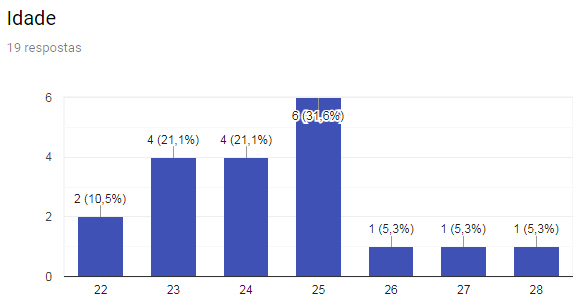
\includegraphics[width=0.75\textwidth]{figuras/avaliacao/idade.png}
        \end{center}
    \label{avalGrafIdade}
    \legend{Fonte: Autor}
\end{figure}    

\begin{figure}[h]
    \caption{Grau de escolaridade dos voluntários.}
       	\begin{center}
            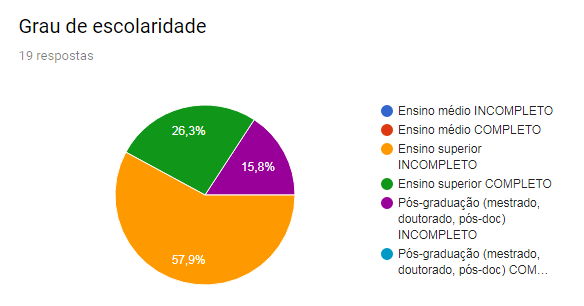
\includegraphics[width=0.75\textwidth]{figuras/avaliacao/escolaridade.png}
        \end{center}
    \label{avalGrafEscolaridade}
    \legend{Fonte: Autor}
\end{figure} 

\begin{figure}[H]
    \caption{Áreas de formação superior dos voluntários.}
       	\begin{center}
            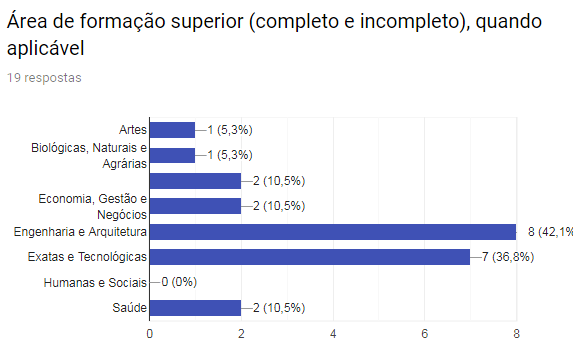
\includegraphics[width=0.75\textwidth]{figuras/avaliacao/area-formacao.png}
        \end{center}
    \label{avalGrafAreasAtuacao}
    \legend{Fonte: Autor}
\end{figure} 

\begin{figure}[h]
    \caption{Experiência dos voluntários com Internet.}
       	\begin{center}
            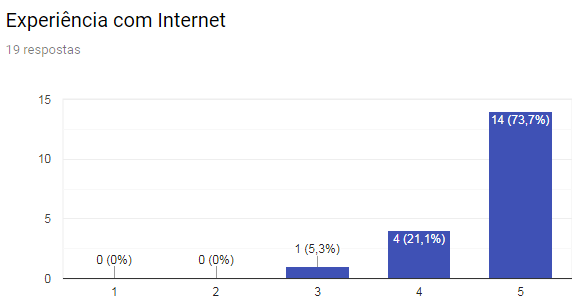
\includegraphics[width=0.75\textwidth]{figuras/avaliacao/xp-internet.png}
        \end{center}
    \label{avalGrafInternet}
    \legend{Fonte: Autor}
\end{figure} 

\begin{figure}[H]
    \caption{Experiência dos voluntários com redes sociais.}
       	\begin{center}
            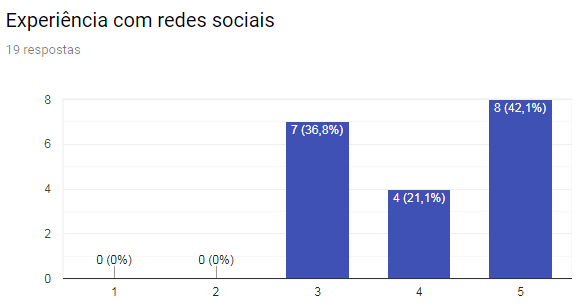
\includegraphics[width=0.75\textwidth]{figuras/avaliacao/xp-redes-sociais.png}
        \end{center}
    \label{avalGrafRedesSociais}
    \legend{Fonte: Autor}
\end{figure} 

\begin{figure}[H]
    \caption{Experiência dos voluntários com a rede social LinkedIn.}
       	\begin{center}
            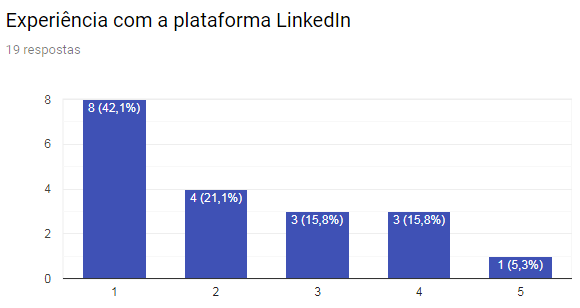
\includegraphics[width=0.75\textwidth]{figuras/avaliacao/xp-linkedin.png}
        \end{center}
    \label{avalGrafLinkedin}
    \legend{Fonte: Autor}
\end{figure}

\begin{figure}[H]
    \caption{Experiência dos voluntários com a plataforma Mural de Bolsas da UFRGS.}
       	\begin{center}
            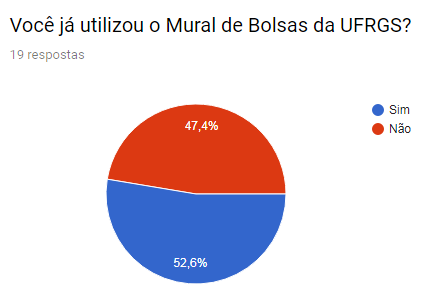
\includegraphics[width=0.7\textwidth]{figuras/avaliacao/mural-bolsas.png}
            \\
            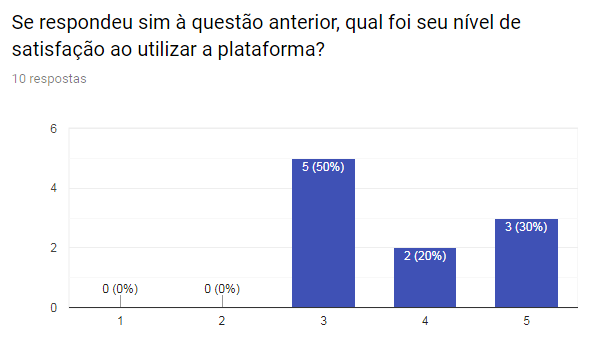
\includegraphics[width=0.8\textwidth]{figuras/avaliacao/mural-bolsas-2.png}
        \end{center}
    \label{avalGrafMB}
    \legend{Fonte: Autor}
\end{figure}

\section{Análise geral dos resultados}
\label{avaliacaoAnalise}

Os resultados avaliados serão divididos em duas categorias: resultados dos teste A/B e resultados do teste de usabilidade. O primeiro avalia as respostas e opinião dos participantes nos questionários em questões que comparam funcionalidades presentes no Mural de Bolsas e Portal de Vagas. Já o segundo avalia as respostas e opiniões em soluções implementadas exclusivamente no Portal de Vagas.


\subsection{Análise Teste A/B}
\label {avaliacaoAnaliseSubjetiva}

Analisando as respostas obtidas durante a primeira etapa do teste, sobre o questionário de caracterização dos voluntários, podemos destacar alta escolaridade em várias áreas de formação, bastante experiência com a Internet, redes sociais, pouco contato com a rede social LinkedIn e uma distribuição quase igual de participantes que já utilizaram o Mural de Bolsas dos que não o tinham usado até o momento da avaliação. 

Esses resultados já eram esperados e o questionário foi feito justamente com o intuito de englobar um nicho de participantes genérico, isto é, sem ter obrigatoriamente um grande conhecimento em tecnologias ou ser de uma área de formação específica, visto que, aplicações como redes sociais possuem uma grande diversidade de usuários. Logo, nenhum participante foi descartado a partir das respostas fornecidas nesta etapa.

Ao final de cada sequência de atividades propostas numa plataforma, foi aplicado um questionário para o participante informar o nível de dificuldade das tarefas. Como foi utilizado o protocolo de teste A/B, um grupo de usuários realizou o experimento primeiro com o Portal de Vagas e, posteriormente, o Mural de Bolsas. O outro grupo realizou o experimento na ordem inversa. Nesta etapa, em cada uma das plataformas, existiam duas perguntas referentes a telas e navegação do sistema. Caso algum usuário respondesse pelo menos uma dessas questões erradas, seria desclassificado, pois se assumiria que este não dedicou a atenção necessária durante o experimento. Contudo, não houve descarte de nenhuma participação de todos os 19 voluntários.

Sendo assim, um número maior de voluntários achou a realização das tarefas no Portal de Vagas muito mais fácil do que no Mural de Bolsas, apesar da plataforma ter recebido uma única avaliação indicando que as tarefas foram muito difíceis. De modo geral, o Portal de Vagas apresentou uma avaliação média maior que o Mural de Bolsas (4,47 e 4,26 respectivamente) e também um desvio padrão maior (0,93 contra 0,78). A Figura \ref{avalGrafABDesemp} apresenta o total de cada nota atribuída pelos voluntários no questionário em cada uma das plataformas.

\begin{figure}[ht]
    \caption{Dificuldade dos voluntários na realização das tarefas propostas nas duas plataformas, onde, no eixo X do gráfico, a avaliação 1 equivale a "muito difícil e, 5 "muito fácil".}
       	\begin{center}
            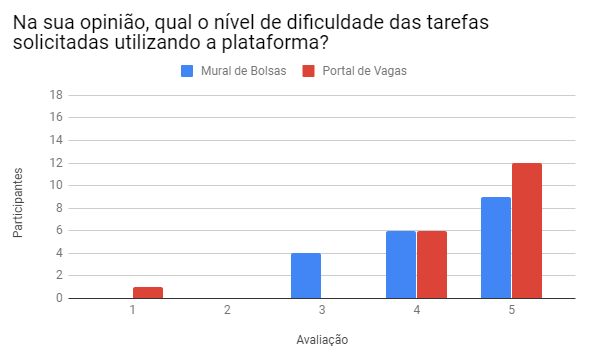
\includegraphics[width=0.85\textwidth]{figuras/avaliacao/ab-dificuldade.png}
        \end{center}
    \label{avalGrafABDesemp}
    \legend{Fonte: Autor}
\end{figure} 

\begin{figure}[H]
    \caption{Satisfação dos voluntários na realização das tarefas propostas nas duas plataformas, onde avaliação 1 equivale a "muito mal" e, 5 "muito bem".}
       	\begin{center}
            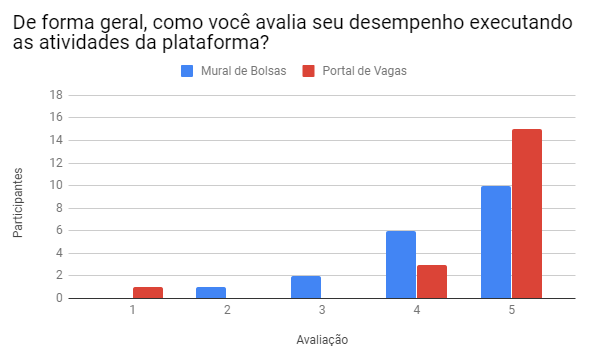
\includegraphics[width=0.85\textwidth]{figuras/avaliacao/ab-desempenho.png}
        \end{center}
    \label{avalGrafABSatisfacao}
    \legend{Fonte: Autor}
\end{figure} 

\subsection{Teste de usabilidade}
\label {avaliacaoUsabilidade}

Complementarmente às tarefas solicitadas em comum nas duas aplicações, quando o voluntário estava no Portal de Vagas, ele realizava algumas tarefas adicionais com o intuito de avaliar a usabilidade de funcionalidades que não existem no Mural de Bolsas. Dessa forma, podemos deduzir se os incrementos na plataforma são válidos e intuitivos para os usuários finais.

Para cada uma das tarefas solicitadas, uma questão de escala linear era proposta perguntando qual a dificuldade do voluntário ao realizá-la. Em todas as questões dessa seção do formulário, o valor 1 corresponde a "muito difícil" e 5, "muito fácil". De modo geral, todas as atividades tiveram como maioria das respostas uma avaliação de "muito fácil". Contudo, alguns casos interessantes foram constatados. 

As atividades de curtir e comentar, ficaram com a média mais baixa entre todas avaliadas. Isto ocorreu, segundo os comentários dos voluntários, porque a navegação até a página com essas informações não é intuitiva em um primeiro momento. Logo, a experiência foi comprometida até que eles tivessem um domínio maior desta funcionalidade na rede social. A Figura \ref{avalGrafTUCurtir} apresenta os valores aplicados pelos usuários à questão do formulário.

\begin{figure}[h]
    \caption{Dificuldade dos voluntários na realização das tarefas de curtir e comentar em postagens.}
       	\begin{center}
            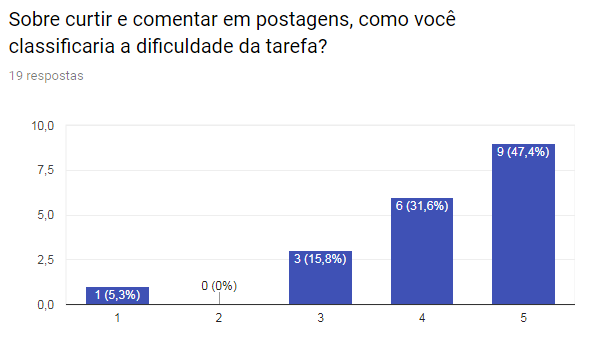
\includegraphics[width=0.75\textwidth]{figuras/avaliacao/pdv-4.png}
        \end{center}
    \label{avalGrafTUCurtir}
    \legend{Fonte: Autor}
\end{figure} 


A atividade de atualizar foto de perfil, seguida pelas de pesquisar usuários e vagas, foram as melhores avaliadas, como é possível observar nas Figuras \ref{avalGrafTUPerfil} e \ref{avalGrafTUPesquisar}. Isto ocorreu porque, para a foto de perfil, havia uma mensagem em formato de alerta bastante convidativa que instruía o usuário a completar essa informação do perfil. Quanto à pesquisa, o formulário fixo no cabeçalho das páginas, bastante comum nos dias atuais em mecanismos de busca, facilitou a localização dos voluntários no sistema, tornando a tarefa bastante natural.

\begin{figure}[h]
    \caption{Dificuldade dos voluntários na realização da tarefa de atualizar foto de perfil.}
       	\begin{center}
            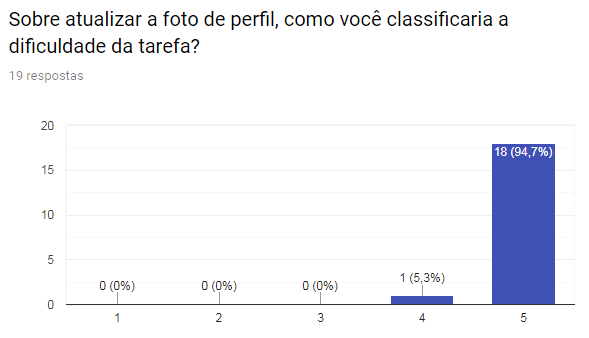
\includegraphics[width=0.75\textwidth]{figuras/avaliacao/pdv-1.png}
        \end{center}
    \label{avalGrafTUPerfil}
    \legend{Fonte: Autor}
\end{figure} 

\begin{figure}[H]
    \caption{Dificuldade dos voluntários na realização da tarefa de pesquisar usuários e vagas.}
       	\begin{center}
            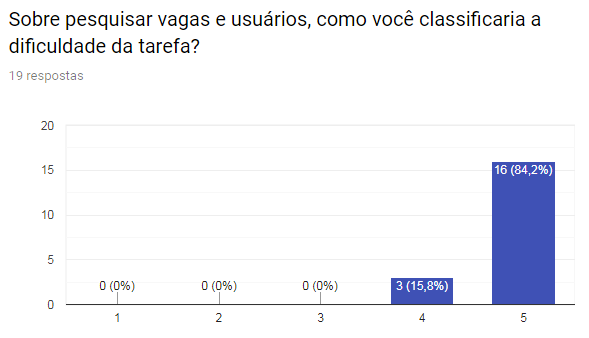
\includegraphics[width=0.75\textwidth]{figuras/avaliacao/pdv-5.png}
        \end{center}
    \label{avalGrafTUPesquisar}
    \legend{Fonte: Autor}
\end{figure} 


Vários usuários alegaram que a tarefa de preencher perfil foi onerosa. Segundo eles, não houve problema para achar a página e, de fato, preencher o perfil. Contudo, por apresentar vários formulários para preenchimento, a finalização dessa atividade foi cansativa.

\begin{figure}[H]
    \caption{Dificuldade dos voluntários na realização da tarefa de preencher dados do perfil.}
       	\begin{center}
            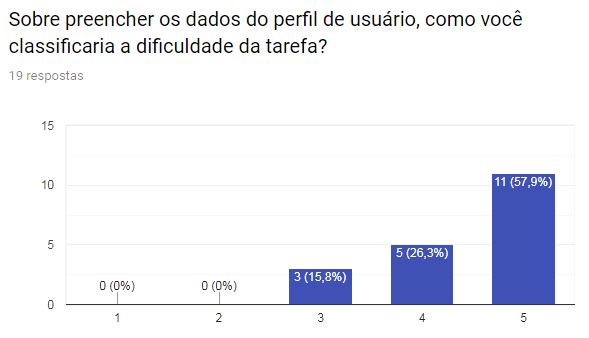
\includegraphics[width=0.75\textwidth]{figuras/avaliacao/pdv-2.png}
        \end{center}
    \label{avalGrafTUPreencherPerfil}
    \legend{Fonte: Autor}
\end{figure} 

A tarefa de seguir os usuários obteve uma avaliação bem alta. Os principais motivos que levaram a tarefa contemplar tamanha aceitação dos usuários foi a disponibilização de vários áreas do site com botões intuitivos para seguir listas de usuários que eram apresentadas. Portanto, completar o objetivo solicitado ficou natural durante a navegação do usuário pela rede social. A Figura \ref{avalGrafTUSeguir} apresenta o resultado das avaliações coletadas.

\begin{figure}[h]
    \caption{Dificuldade dos voluntários na realização da tarefa de seguir usuários.}
       	\begin{center}
            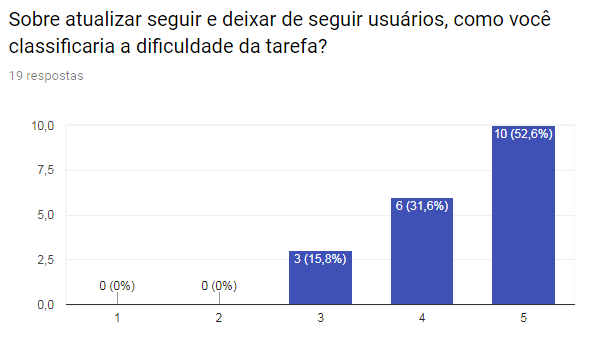
\includegraphics[width=0.75\textwidth]{figuras/avaliacao/pdv-3.png}
        \end{center}
    \label{avalGrafTUSeguir}
    \legend{Fonte: Autor}
\end{figure} 

Por fim, a recomendação de usuários e vagas também foi uma tarefa bem avaliada pelos voluntários. Alguns comentários recebidos indicaram uma dificuldade de navegação no sistema até achar a funcionalidade, mas, uma vez encontrada, ela é basante amigável e encoraja a pessoa a utilizá-la. A Figura \ref{avalGrafTURecomendar} exibe as avaliações recebidas da funcionalidade no questionário aplicado.

\begin{figure}[H]
    \caption{Dificuldade dos voluntários na realização da tarefa de recomendar usuários e vagas.}
       	\begin{center}
            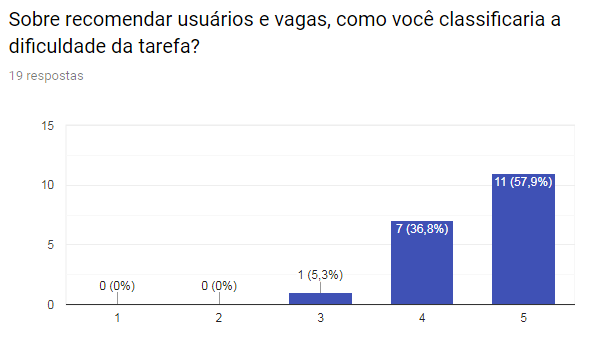
\includegraphics[width=0.75\textwidth]{figuras/avaliacao/pdv-6.png}
        \end{center}
    \label{avalGrafTURecomendar}
    \legend{Fonte: Autor}
\end{figure}